\section{Analysis}
\label{sec:analysis}

The main experiments show that RACES improves generalization.
Further analysis is conducted to evaluate RACES's performance.
All analysis experiments are conducted on Qwen3-4B-Instruct-2507 to reduce computational cost.

\subsection{Performance across Training Process}
\label{sec:training_dynamic}

We first compare the training dynamics of $RL_{RACES}$ and $RL_{individual}$ on Qwen3-4B-Instruct-2507.
A natural expectation is that a method that increases reward more rapidly during reinforcement learning will also achieve superior downstream generalization.
However, the results indicate that this expectation does not hold. Figure~\ref{fig:training_dynamic} compares the training reward and average performance during RL training.
$RL_{individual}$ improves more rapidly and maintains consistently higher rewards throughout training, suggesting that the model adapts more easily to environments.
In contrast, $RL_{RACES}$ exhibits progressively slower reward growth, reflecting the increased complexity of composite environments.

However, the advantage of $RL_{individual}$ in training reward does not result in superior downstream performance.
As shown in Figure~\ref{fig:training_ood}, the average score of $RL_{individual}$ improves fast at the beginning, and then quickly peaks around 50.5.
Conversely, $RL_{RACES}$ continues to improve throughout the training process. While initially comparable to $RL_{individual}$, it gradually surpasses $RL_{individual}$ after the early stages, reaching 51.9 at step 200 compared to 50.4.

These findings differentiate between overfitting to training environments and acquiring transferable reasoning behaviors.
Individual environments are shorter and structurally simpler, making them easier to optimize and leading to rapid reward gains.
However, this improvement remains largely restricted to the training distribution.
Composite environments in RACES require the model to maintain intermediate states, execute multi-step transformations, and, in some cases, infer the latent order of operations.
Although these tasks are more challenging and result in slower reward improvement, they offer a richer training signal and produce more sustained gains on downstream benchmarks.
This suggests that the primary advantage of RACES is the induction of reasoning patterns that generalize more effectively beyond the training environments.

\begin{figure}[t]
\centering
\begin{subfigure}[t]{0.42\textwidth}
\centering
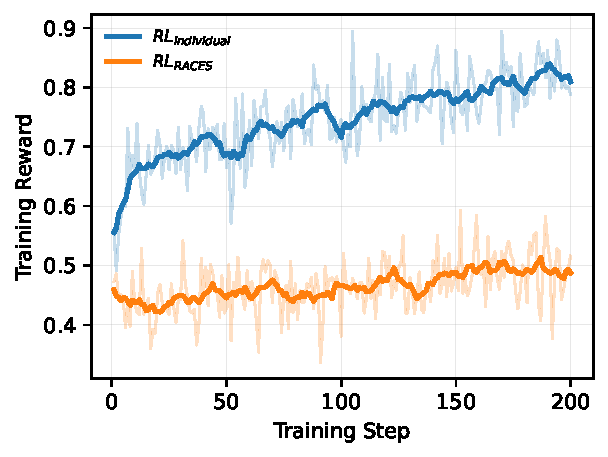
\includegraphics[width=\linewidth]{Figures/training_reward_panel.pdf}
\caption{Training Rewards.}
\label{fig:training_dynamic}
\end{subfigure}
\hspace{10px}
\begin{subfigure}[t]{0.42\textwidth}
\centering
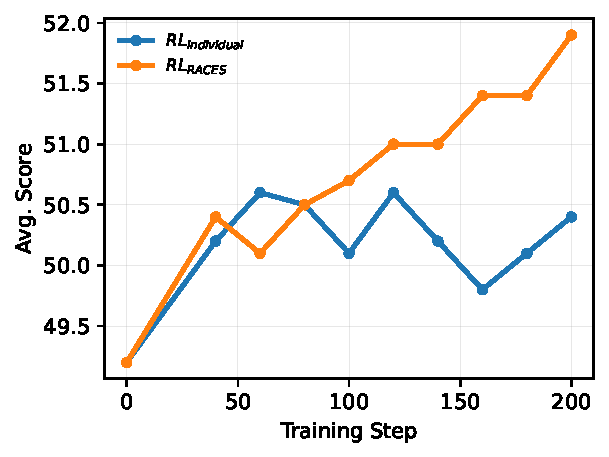
\includegraphics[width=\linewidth]{Figures/ood_performance_panel.pdf}
\caption{Average performance across the training process.}
\label{fig:training_ood}

\end{subfigure}
\caption{\textbf{Training dynamics on Qwen3-4B-Instruct-2507.} \emph{(a)} Smoothed training reward over $200$ RL steps. \emph{(b)} Average performance.}
\vspace{-8pt}

\end{figure}

\subsection{Efficiency of Environment Utilization}
\label{sec:efficiency}

\begin{table}[!t]
\centering
\caption{Results of RACES and individual RL on the initial environment pool with different sizes.}
\resizebox{0.8\linewidth}{!}{
\begin{tabular}{lcccccc}
\toprule
Setting & LCB & Enigmata & LBench-V2 & IFEval & AIME & Avg. \\
\midrule
\multicolumn{7}{l}
{\textcolor{gray}{\textit{Qwen3-4B-Instruct-2507 as base model}}}\\
\noalign{\vskip 0.11cm}
\textsc{BASE} & 32.4 & 36.5 & 41.3 & 82.2 & 53.7 & 49.2 \\
$RL_{individual}$ (50 envs)  & 32.7 & 38.6 & 41.6 & 82.9 & 55.1 & 50.2  \\
$RL_{individual}$ (300 envs) & 31.5 & 39.3 & 41.9 & 83.5 & 55.6 & 50.4  \\
$RL_{RACES}$ (50 envs)       & 33.2 & 38.7 & 42.4 & 82.8 & 57.0 & 50.8  \\
$RL_{RACES}$ (300 envs)      & \textbf{34.0} & \textbf{39.5} & \textbf{42.7} & \textbf{85.2} & \textbf{58.3} & \textbf{51.9} \\
\noalign{\vskip 0.11cm}
\hdashline
\noalign{\vskip 0.11cm}
\multicolumn{7}{l}
{\textcolor{gray}{\textit{DeepSeek-R1-Distill-Qwen-14B as base model}}}\\
\noalign{\vskip 0.11cm}
\textsc{Base} & 47.2 & 32.3 & 32.5 & 70.6 & 58.5 & 48.2 \\
$RL_{individual}$ (300 envs) & 46.9 & 34.2 & 33.7 & 69.3 & 59.8 & 48.8 \\
$RL_{RACES}$ (50 envs)       & \textbf{47.4} & \textbf{34.7} & \textbf{35.7} & \textbf{73.0} & \textbf{60.3} & \textbf{50.2} \\
\bottomrule
\end{tabular}
}
\label{tab:env_efficiency}
\vspace{-10pt}
\end{table}

The results in Figure \ref{fig:training_ood} indicate that $RL_{RACES}$ significantly outperforms $RL_{individual}$ when both are provided with the same 300 initial environments.
Further analysis examines whether RACES maintains this advantage across varying numbers of environments.

Table~\ref{tab:env_efficiency} compares the performance of Qwen3-4B-Instruct-2507 on 50 and 300 initial environments, denoted as $RL_{setting}(50)$ and $RL_{setting}(300)$
$RL_{individual}$ improves the average score from 49.2 to 50.2 and rises to 50.4 when utilizing all 300 environments.
In contrast, $RL_{RACES}(50)$ achieves 50.8, outperforming $RL_{individual}(300)$ with only one-sixth of the base environment pool.
$RL_{RACES}(300)$ further increases to 51.9.
The same trend appears on DeepSeek-R1-Distill-Qwen-14B. $RL_{RACES}(50)$ reaches 50.2, clearly above $RL_{individual}(300)$ at 48.8.

This substantial difference demonstrates that RACES enhances the efficiency of environment utilization.
An individual environment can provide only instances of a single transformation family.
However, once composed, the same environment can appear at different positions, with different neighboring environments, under different operators.
Thus, composition converts a fixed environment pool into a much larger and structurally more diverse training distribution.
This represents the principal advantage of RACES over linear environment scaling, as it increases the utility of each existing environment rather than relying exclusively on synthesizing additional independent environments.

\subsection{Effect of Composition Size}
\label{sec:composition_size}

The effect of composition size on training effectiveness is subsequently examined.
Composition size is a central control variable in RACES, increasing it does not merely change the amount of generated data but directly changes the structure and difficulty of the resulting composite environments.
Larger compositions require the model to maintain more intermediate states, handle longer dependency chains, and tolerate stronger error propagation, thereby increasing the overall reasoning burden.

To isolate this effect, the environment pool is fixed at $|\mathcal{E}|=300$, and variants with different composition sizes are trained on Qwen3-4B-Instruct-2507.
The analysis focuses on the \textsc{SEQUENTIAL} operator, for which composition size has the most direct interpretation, and varies the size from 2 to 6.
Figure~\ref{fig:composition_size} summarizes both the training dynamics and the final performance under different composition sizes.

The training curves reveal a clear increase in optimization difficulty as composition size grows.
As shown in Figure~\ref{fig:composition_size}(a), the rewards are consistently higher for smaller composition sizes and decrease as the size increases, indicating that deeper compositions are harder for the policy to optimize.
A similar trend is observed in Figure~\ref{fig:composition_size}(b). The average reward variance (affecting advantage directly) tends to be lower for larger composition sizes, suggesting that deeper compositions leave a less informative learning signal for RL.

The effect on downstream performance is shown in Table~\ref{tab:composition_size}.
As the composition size increases from 2 to 5, the average score improves steadily from 50.8 to 51.2.
However, when the size is increased further to 6, performance decreases to 50.7.
This produces a clear non-monotonic trend. Increasing composition size is beneficial up to a moderate-to-large range, but excessively deep compositions become less effective.
Taken together, these results reveal a trade-off between reasoning generalization and trainability.
Small composition sizes are easier to optimize, but they provide only limited expansion beyond environments.
Increasing the composition size introduces richer multi-step reasoning patterns and improves reasoning generalization.
However, once the composition becomes too deep, the difficulty of optimization begins to dominate: rewards decrease, reward variance becomes less informative, and final performance deteriorates.
In practice, these results suggest that composition size should be regarded as a controllable curriculum variable rather than a parameter to maximize indiscriminately.

% \begin{figure}
%     \centering
%     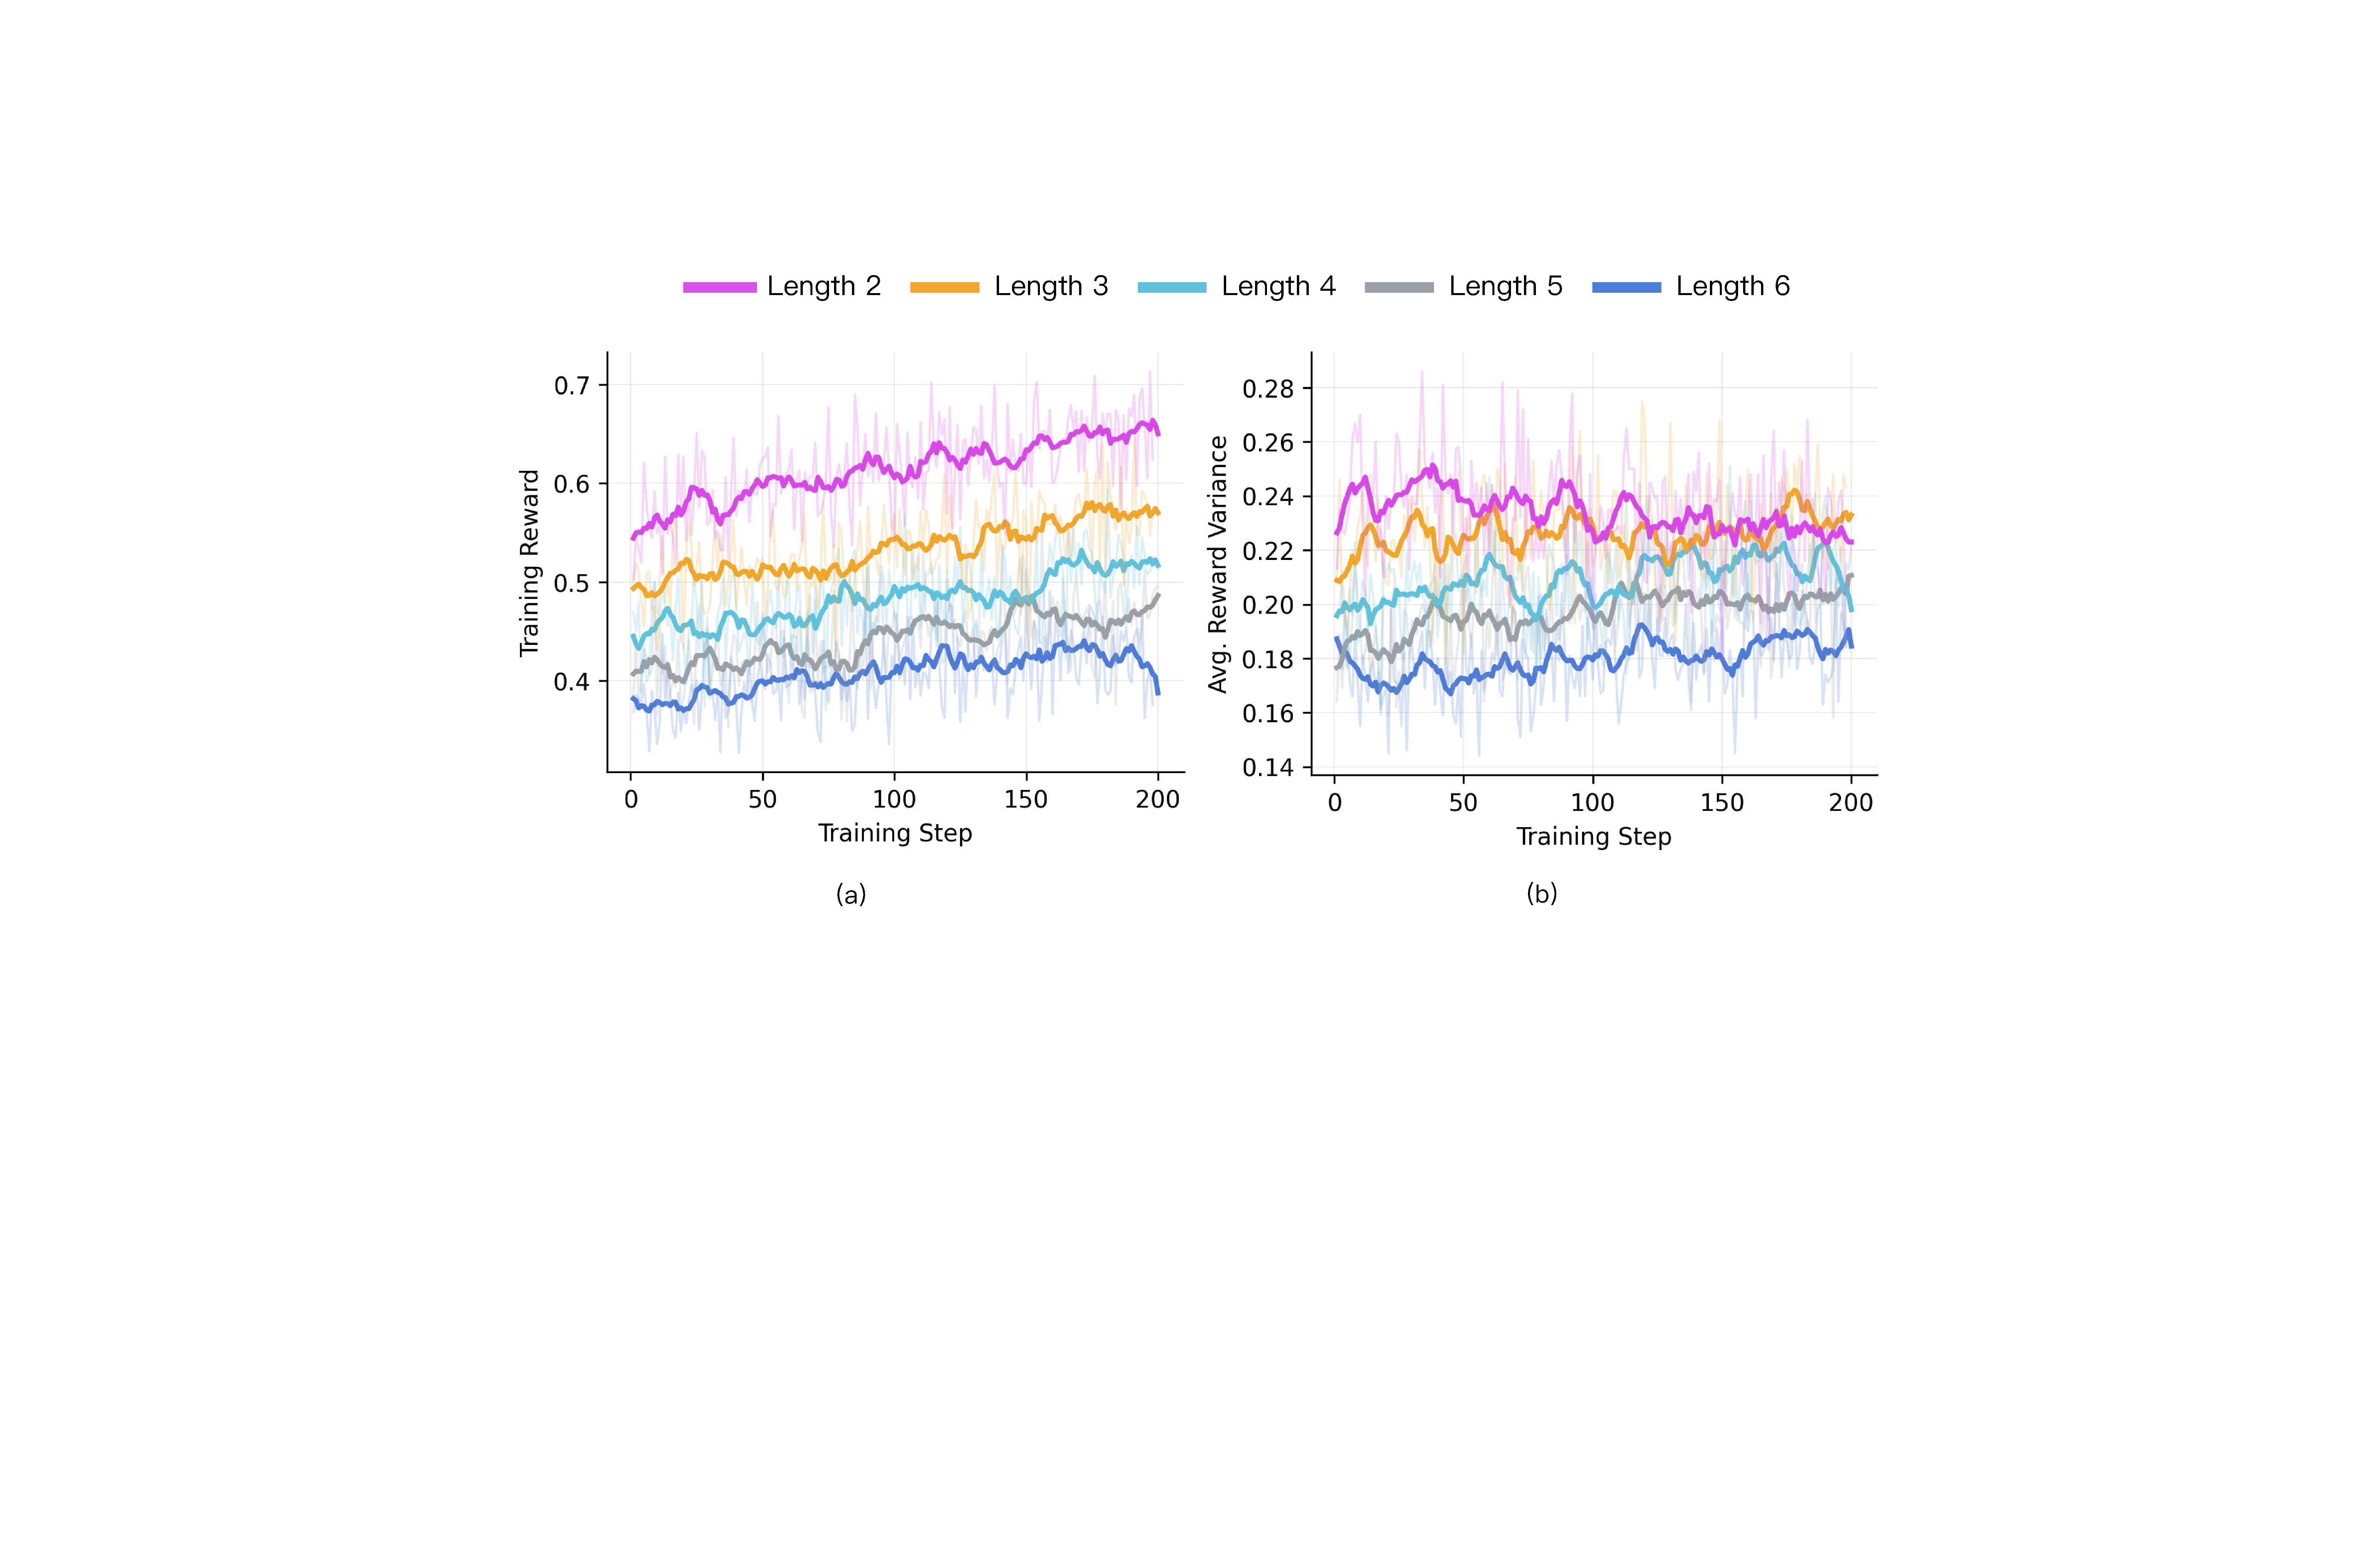
\includegraphics[width=0.8\linewidth]{Figures/length.pdf}
%     \caption{\textbf{Effect of composition size for the \textsc{Sequential} operator on Qwen3-4B-Instruct-2507}, with $|E|!=!300$ environments fixed. \emph{(a)} rewards during training. \emph{(b)} Average reward variance, the mean of every problem’s rollout reward std.}
%     \label{fig:composition_size}
% \end{figure}

\begin{figure}
\centering
\begin{minipage}[t]{0.75\linewidth}
\vspace{0pt}
\centering
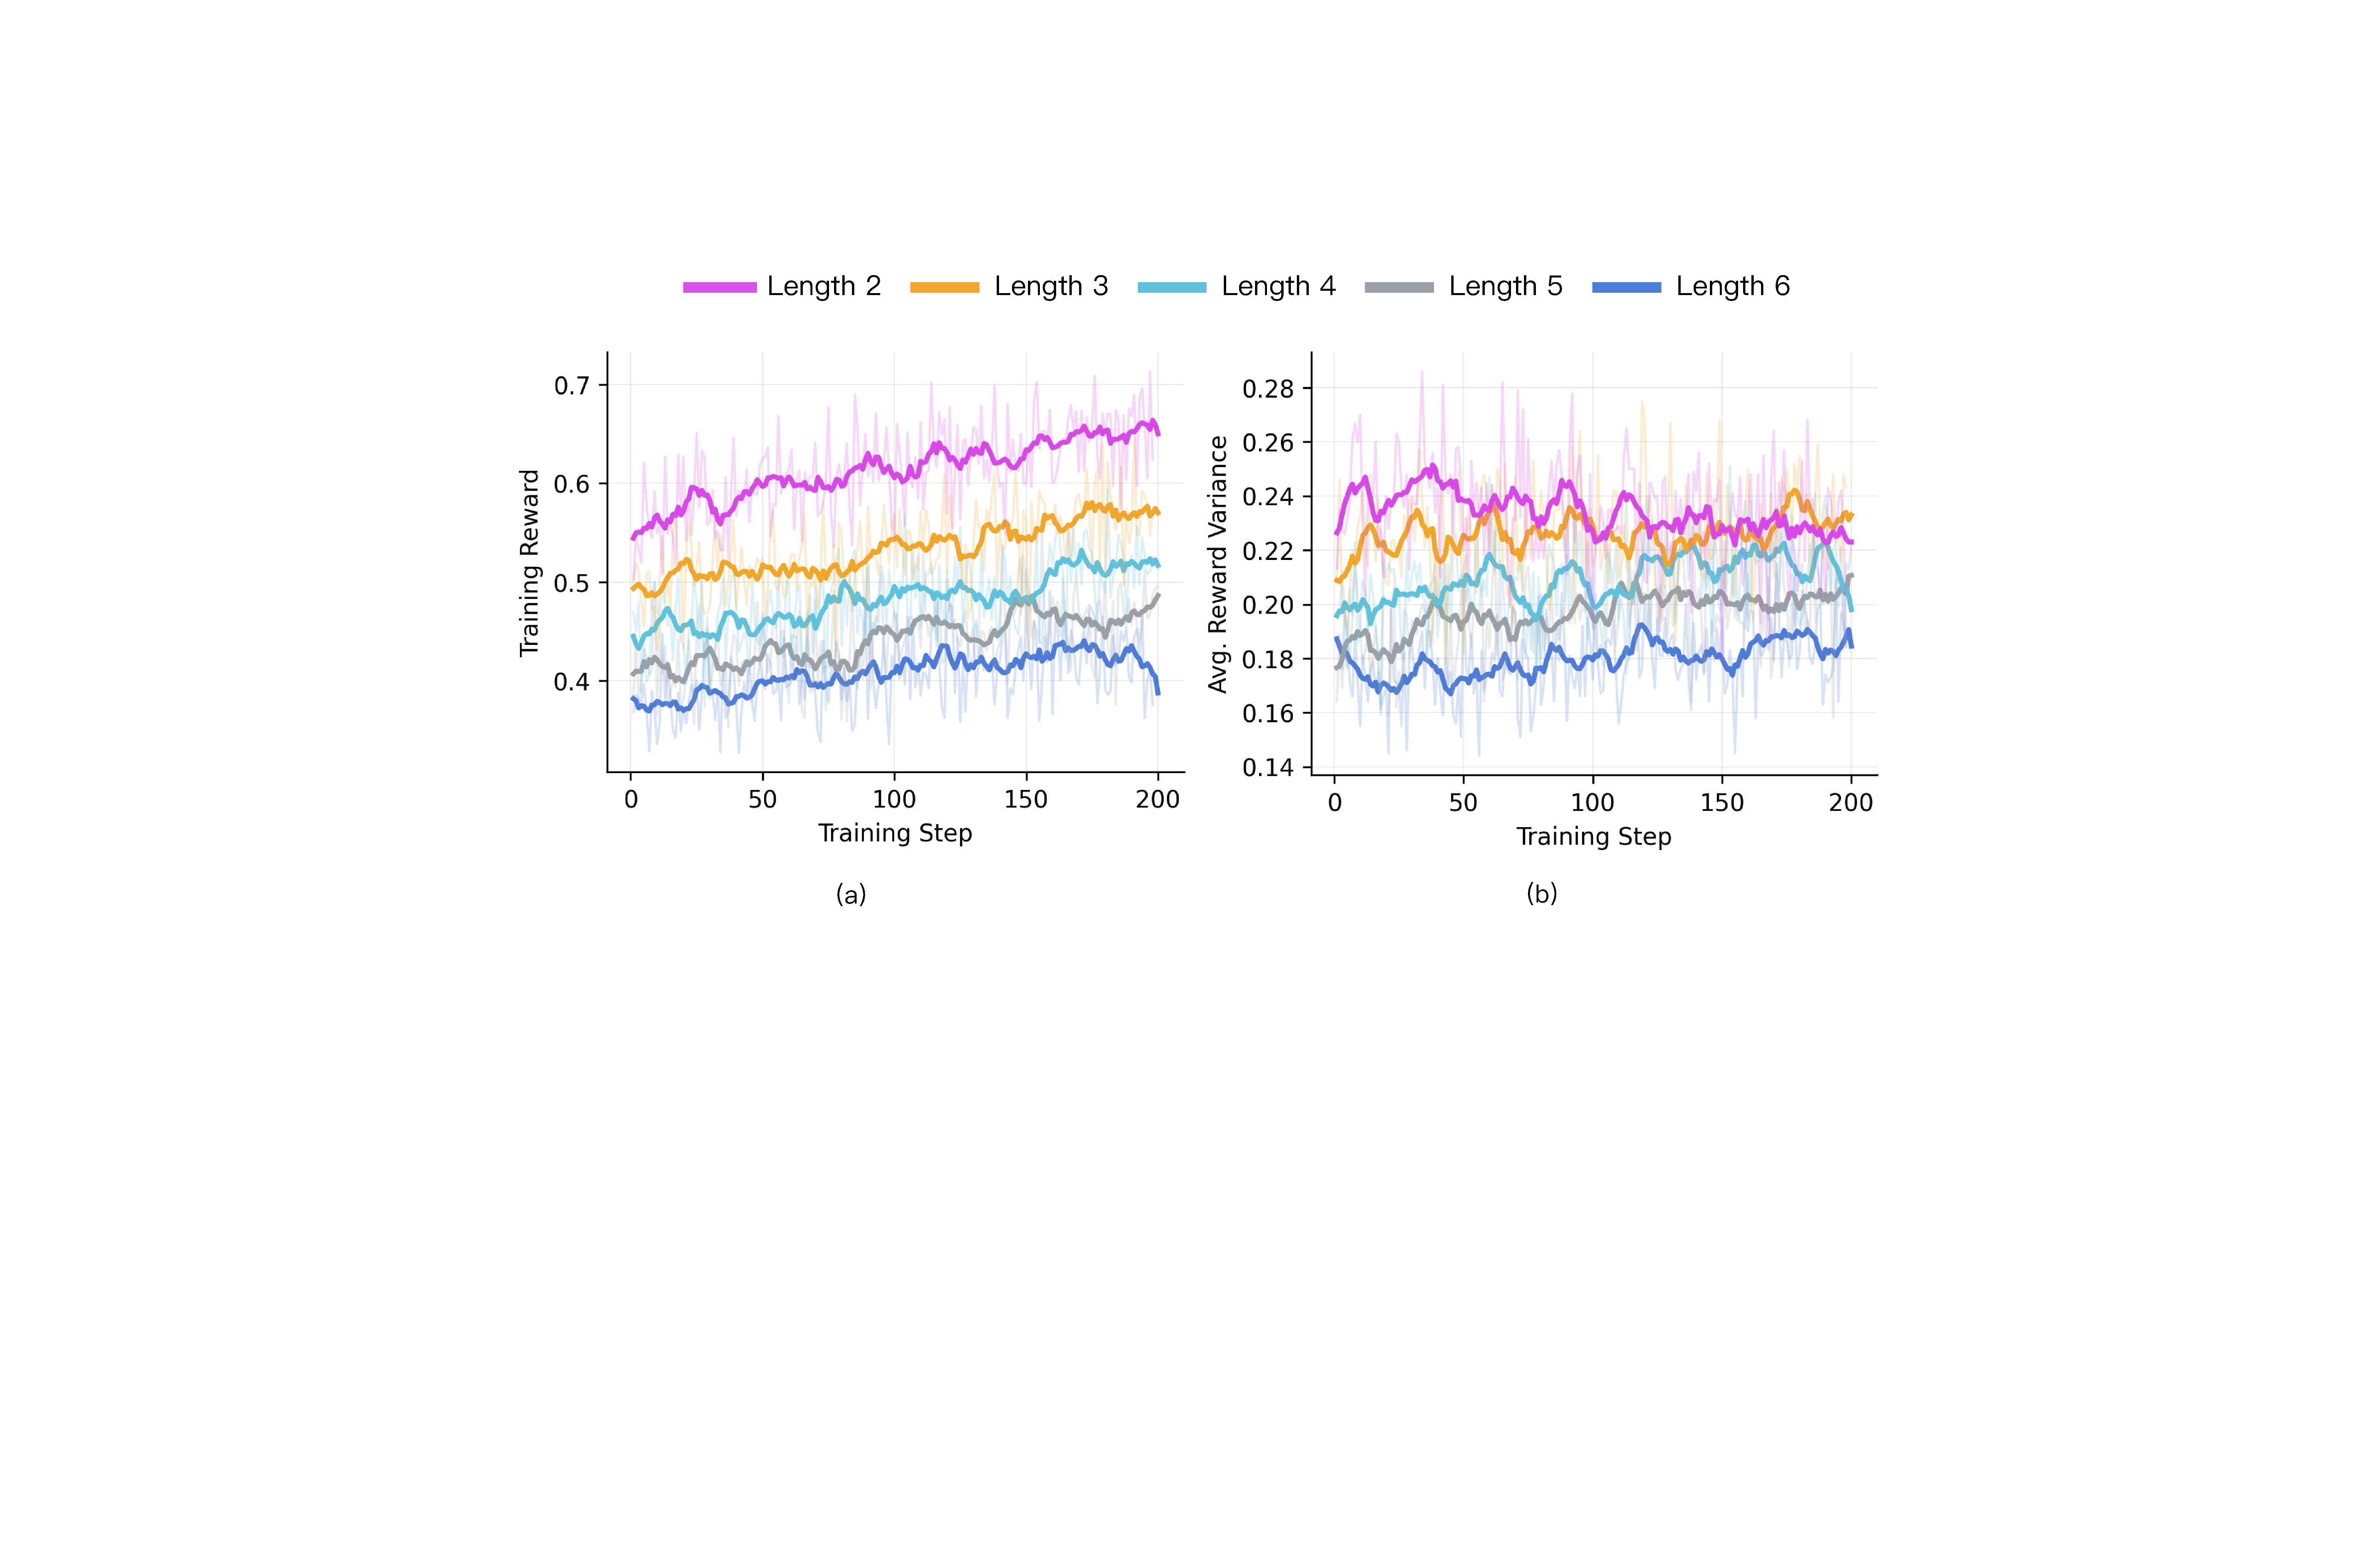
\includegraphics[width=\linewidth]{Figures/length.pdf}
\caption{Effect of composition size. \emph{(a)} rewards during training. \emph{(b)} Average reward variance, the mean of every problem’s rollout reward std.}
\label{fig:composition_size}
\end{minipage}\hfill
\begin{minipage}[t]{0.23\linewidth}
\vspace{0pt}
\centering
\captionof{table}{Average scores under different sizes.}
\label{tab:composition_size}
\small
\begin{tabular}{cc}
\toprule
Size & Performance \\
\midrule
2 & 50.8 \\
3 & 50.7 \\
4 & 51.0 \\
5 & \textbf{51.2} \\
6 & 50.7 \\
\bottomrule
\end{tabular}
\end{minipage}
\end{figure}

\subsection{Pattern Analysis}
\label{sec:pattern_analysis}

To complement the aggregate results, qualitative comparisons are made between responses from the base model, $RL_{individual}$, and $RL_{RACES}$ on identical AIME and Enigmata prompts. Three representative cases are presented in Appendix~\ref{app:cases}.

For AIME. In the $2{\times}2$ grid-coloring problem (Appendix~\ref{app:case-grid-coloring}), the base model sets up a valid enumeration but confuses variables when filling the case table and $RL_{individual}$ makes a single inconsistent update on an internal edge color. Both errors are local yet propagate to the final count. The $RL_{RACES}$ model instead introduces a compact function $f(x,y)$ that maps each pair of internal-edge colors to its boundary-assignment count, applies it uniformly, and cross-checks the total via an independent grouping calculation—replacing error-prone table-filling with representation-mediated counting and self-consistency verification.

For Enigmata. In a list-transformation task (Appendix~\ref{app:case-list-transform}), the base model and $RL_{individual}$ both cycle through surface rules (suffix extraction, duplicate-run selection) without rejecting hypotheses that fail earlier examples and $RL_{individual}$ even notes a contradiction yet continues with the falsified rule. The $RL_{RACES}$ model maintains explicit index–value tracking, tests each candidate against all demonstrations, and identifies the correct rule. A related pattern appears on Sum Skyscraper (Appendix~\ref{app:case-skyscraper}), non-RACES models commit to an incomplete row-wise search and reach a spurious “no valid solution.” $RL_{RACES}$ reframes the search column-by-column, exhausts a smaller space, propagates fixed values through row-uniqueness, and verifies all 16 clues.

These behaviors reflect the RACES training signal. \textsc{SEQUENTIAL} compositions train state carry-over, \textsc{Parallel} compositions train subproblem separation, \textsc{Sort} compositions train order inference, and \textsc{Select} introduces distractor discrimination. The transferable routines, including stable intermediate representations, constraint preservation, hypothesis revision, and final-answer verification, account for the observed performance gains without requiring surface similarity to the training environments.